% ----- preamble -----
% {{{
\documentclass[11pt]{article}

% page geometry, margins and figures
\usepackage{geometry}
\geometry{letterpaper, portrait, margin=0.60in}

% color and figures
\usepackage{wrapfig}
\usepackage[usenames,dvipsnames]{xcolor}
\usepackage{graphicx}
\usepackage{pdfpages} % for including pdfs into proposal
\usepackage{tikz}
\usetikzlibrary{positioning}
\definecolor{lightorange}{HTML}{fff2cc}
\definecolor{lightblue}{HTML}{b3d2ff}

% Math and chemistry packages
\usepackage{amsmath, amssymb}
\usepackage{bm}
\DeclareMathOperator{\tr}{tr}
\usepackage[version=4]{mhchem}
\usepackage{textgreek}

% font and paragraph spacing
\setlength{\parindent}{0pt} % no indent
\setlength{\parskip}{0.30\baselineskip} % adjust length a bit more; narrow = 0.25; wider = 0.34
\renewcommand{\baselinestretch}{0.95} % NSF PAPPG allows 54 lines per 9 in page (6 lines/in). 0.88 gives this.
\usepackage[T1]{fontenc}
\usepackage[utf8]{inputenc}
\usepackage{microtype} % magic package that fixed the problem with my reference in the margin!!
\renewcommand{\familydefault}{\sfdefault} % for sans serif font

% --- bibliography ---
\usepackage[style=numeric-comp, eprint, backend=biber, doi=true,
            maxbibnames=99, sorting=none, isbn=false]{biblatex}
\renewbibmacro{in:}{}
\addbibresource{refs.bib}
\let\cite=\supercite

% allow reference without brackets
\DeclareCiteCommand{\citenum}
  {}
  {\printfield{labelnumber}}
  {}
  {}

% --- Format title/authors ---
% \usepackage{titling}
% \pretitle{ {\Large\textbf{W{\normalsize{}HITE} P{\normalsize{}APER} | C{\normalsize{}ONFIDENTIAL} }} \par\vspace{1em}\LARGE\bfseries}
% \posttitle{\par\vspace{0.5em}}
% \preauthor{\large}
% \postauthor{\par\vspace{1.5em}}

% \date{} % no date in title, put in footnote
% \predate{}
% \postdate{}

\usepackage{authblk} % https://ctan.math.utah.edu/ctan/tex-archive/macros/latex/contrib/preprint/authblk.pdf
\renewcommand\Authands{, } % Set the delimiter between authors
\setlength{\affilsep}{1.0em}

% --- Format sections ---
\usepackage{titlesec}
% Reduce spacing around section/subsection titles
\titleformat{\section}{\normalfont\Large\bfseries}{\thesection}{1em}{}
\titlespacing*{\section}{0pt}{1.5ex plus 1ex minus .2ex}{0.5ex plus .2ex}
\titleformat{\subsection}{\normalfont\large\bfseries}{\thesubsection}{1em}{}
\titlespacing*{\subsection}{0pt}{1ex plus 1ex minus .2ex}{0.5ex plus .2ex}

% Caption formatting, make Figure->Fig.
\usepackage[font=small, labelfont=bf, labelsep=period, figurename=Figure]{caption} % caption formatting

% adjust bullets, list spacing to make a bit more compact
\usepackage{enumitem}
\setlist[itemize]{leftmargin=2.5ex, label=\raisebox{0.25ex}{\tiny$\bullet$}, parsep=0.25ex}

% --- Format header and footer ---
\usepackage{fancyhdr} % add/modify header & footer
\pagestyle{fancy}
\fancyhf{} % sets both header and footer to nothing
\renewcommand{\headrulewidth}{0pt}
\fancyhead[L]{\nouppercase{\papertitle}}
\lhead{ \small\color{gray}W{\scriptsize{}HITE} P{\scriptsize{}APER} | C{\scriptsize{}ONFIDENTIAL}\par{}}
\chead{ \small\color{gray}}
\rhead{
\includegraphics[width=5.0cm]{figs/BYUEng_Watermark.pdf}\vspace{-1ex}}
\lfoot{ \small\textcolor{gray}\today{}\par}
\rfoot{\thepage}

\date{} % no date in title, put in footnote

% --- Commenting ---
\usepackage{lipsum}
\usepackage{soul}
\newcommand{\rewrite}[1]{{\color{red}#1}}
\newcommand{\edit}[1]{{\color{blue}#1}}
\newcommand{\expand}[1]{{\color{purple}#1}}

\newcommand{\highlight}[1]{{\color{RoyalBlue}#1}}

%Merit Review Criteria 
%(See NSF Proposal & Award Policies & Procedures Guide, Chapter III.A.2.)
%All NSF proposals are evaluated through use of two National Science Board approved merit review criteria listed below. In some instances, however, NSF will employ additional criteria as required to highlight the specific objectives of certain programs and activities. Both criteria are to be given full consideration in the review; each criterion is necessary but neither, by itself, is sufficient.
%As a reviewer you are asked to consider what the proposers want to do, why they want to do it, how they plan to do it, how they will know if they succeed, and what benefits could accrue if the project is successful. These issues apply both to the technical aspects of the proposal and the way in which the project may make broader contributions.
%Please consider the following review elements in your review for the review criteria below:
%•	What is the potential for the proposed activity to:
%o	Advance knowledge and understanding within its own field or across different fields (Intellectual Merit); and
%o	Benefit society or advance desired societal outcomes (Broader Impacts)?
%•	To what extent do the proposed activities suggest and explore creative, original, or potentially transformative concepts?
%•	Is the plan for carrying out the proposed activities well-reasoned, well-organized, and based on a sound rationale? Does the plan incorporate a mechanism to assess success?
%•	How well qualified is the individual, team, or organization to conduct the proposed activities?
%•	Are there adequate resources available to the PI (either at the home organization or through collaborations) to carry out the proposed activities?
%Note that if additional supplementary documents are contained in the proposal, they should be reviewed as part of the Intellectual Merits and Broader Impacts, as appropriate.
% }}}

% ----- document text -----
\begin{document}

\title{A Theory-Driven and Experimentally-Validated Design Framework for Programming the Collective Behavior of Microrobots}
\author[1]{Cameron K. Peterson}
\affil[1]{Electrical and Computer Engineering, Brigham Young University, \textit{ckp3@byu.edu}}
\author[2]{Douglas R. Tree}
\affil[2]{Chemical and Biological Engineering, Brigham Young University}
\author[2]{Joseph Rich}

\maketitle
\thispagestyle{fancy}

\vspace{-2\baselineskip}

% \section*{Introduction}
% {{{

\begin{wrapfigure}[39]{r}{2.15in}
  \centering
  \vspace{-1.0\baselineskip}
  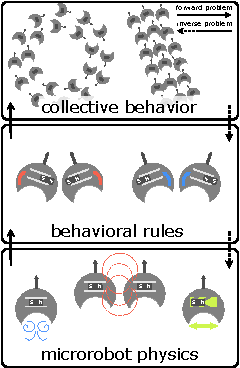
\includegraphics[width=2.15in]{figs/fig-inverse_design_v2.2.pdf}
  \vspace{-19pt}
  \caption{
Proposed framework for the design problem of programmable collective behavior in microrobot swarms.
\textit{Microrobot physics} describes the physical mechanisms governing individual robots (e.g., acoustic streaming, local magnetic interactions, and mechanical logic).
\textit{Behavioral rules} describe coarse-grained local response laws, analogous to local rules in classic flocking and swarming models, that govern how individual robots change their motion, interactions, or internal state in response to neighboring robots or the environment.
\textit{Collective behavior} describes the emergent swarm dynamics (e.g., toroids, swarming) arising from local interactions.
The forward problem predicts collective behavior from the underlying robot physics, while the inverse-design problem seeks to determine the microrobot physics required to realize a desired collective behavior.
  }
  \label{fig-materials}
\end{wrapfigure}

\textbf{Opportunity and Challenge.}
Micro and nanorobotics is a growing field~\cite{Palagi2018} that promises transformative advances in medical technology,~\cite{Sun2019, Koleoso2020, Gumuskaya2023} environmental remediation,~\cite{Maria‐Hormigos2022, Urso2023, Preetam2024, Urso2022} biomimetic and dynamic materials,~\cite{Ling2018, Zhang2019, Parreira2020, Zhao2023} and many other applications.~\cite{Abdoli2022, Hecht2022, Derivaux2023}
However, microscale operation imposes severe physical and computational constraints.
As robots decrease in size, onboard power, sensing, computation, and communication become increasingly limited.
At the same time, robots become strongly coupled to their environment and increasingly susceptible to stochastic disturbances.
Consequently, conventional robotic architectures developed for macroscale systems become fundamentally limited at the microscale.

The hardware constraints imposed at the microscale suggest that robotic intelligence must be distributed rather than centralized. 
Biological collectives from microbial communities to insect swarms demonstrate that sensing, adaptation, transport, and coordinated task execution can emerge from local interactions among large numbers of individually simple agents. 
Applying this paradigm of distributed intelligence to microrobotics offers a scalable alternative to complex individual robots while providing robustness, redundancy, and parallelism that naturally arise from collective operation.

However, this shift from individuals to collectives fundamentally changes the control problem.
Collective behavior emerges from many coupled local interactions, making it difficult to predict, design, and robustly control swarm-level dynamics.
Furthermore, these local interactions depend on robot morphology, material properties, environmental physics, and propulsion and actuation mechanisms, meaning that to date each microrobotic platform requires developing a new mapping from local interactions to collective behavior.
In summary, the central barrier to realizing programmable microrobot swarms is overcoming the highly system-dependent inverse-design problem for predicting and realizing collective behavior.

\textbf{Research Concept.}
The central premise of this work is that the inverse-design problem can be made tractable by introducing an intermediate abstraction layer---behavioral rules---between desired collective behaviors and their physical realization. 
Inspired by classic distributed behavioral models of flocking and swarming, in which simple agent-level rules generate collective motion~\cite{Reynolds1987Boids,Vicsek1995SelfDrivenParticles,Couzin2002CollectiveMemory}, behavioral rules specify coarse-grained local response laws for individual microrobots. 
Operationally, a behavioral rule is a measurable input-output relationship: the change in a robot's motion, interaction, or internal state that results from a specified local configuration of neighboring robots and environmental cues. 
For example, a rule may describe how a robot changes its propulsion direction or internal logic state when a neighboring robot enters a specified range and orientation.

Rather than mapping directly from robot morphology, actuation mechanisms, local interactions, and environmental physics to collective behavior, this intermediate layer decomposes the inverse-design problem into two more tractable subproblems: (i) determining the behavioral rules required to produce a desired collective behavior and (ii) determining how a particular microrobot platform can physically realize those behavioral rules.
In this way, a calibrated library of behavioral rules provides a design framework for microrobotic swarms, enabling physical robot design, reduced-order modeling, and swarm-scale collective behavior to be connected within a common predictive framework.

\textbf{Approach.} %
We will develop Behaviorally Encoded Acoustic Microrobots (BEAMs): 3D-printed, acoustically powered microrobots that combine bistable mechanical logic with programmable magnetic interactions to realize local behavioral rules through physical interactions.
To understand and predict these interactions, we will develop a microscale Brownian dynamics model of BEAMs that captures the local physics of their propulsion, mechanical logic, and neighbor interactions.
In addition to this microscale model, we will use project-operator methods to systematically generate a coarse-grained representation of BEAMs as an Active Brownian Unicycle (ABU).
The reduced-order ABU modeling framework provides a description of behavioral rules and collective behavior that is abstracted from local physics, and can therefore provide a common mathematical language for the inverse design of programmable microrobot swarms.

\textbf{Aims.} %
Realizing this vision requires a framework that connects physical microrobot architecture, coarse-grained local response laws, and emergent collective behavior.
The central objective of this project is to establish this framework by integrating theory, coarse-grained simulation, and experimental realization into a unified approach for designing programmable microrobot swarms. 
To achieve this objective, the proposed research is organized into three tightly coupled aims.

\textbf{Aim 1: Establish a behavioral-rule framework for programmable microrobot swarms.}
Develop theoretical and experimental foundations for representing behavioral rules as coarse-grained local response laws using the ABU framework and BEAMs, establishing a common language for describing local interactions and collective behavior.
We will formulate the ABU framework, develop coarse-graining methods that relate detailed microscale dynamics to behavioral rules, and create first-generation BEAMs that demonstrate the essential capabilities of behavioral-rule microrobots, including acoustic propulsion, stable internal logic states, local magnetic interactions with neighboring robots, and interaction-driven changes in behavior.

\textbf{Aim 2: Connect physical microrobot design to behavioral rules.}
Develop and validate a multiscale modeling framework that identifies how BEAM design parameters and microscale physical interactions give rise to measurable behavioral rules.
We will systematically vary BEAM design parameters (e.g., magnetic interaction strength, acoustic streaming, and compliant mechanical logic) to determine how physical design governs behavioral rules, using iterative comparisons between theory and experiment to refine both the microscale model and the BEAM architecture while demonstrating representative collective behaviors.

\textbf{Aim 3: Demonstrate predictive design of programmable collective behavior.}
Use the validated framework to design new BEAM architectures that realize distinct behavioral rules and demonstrate that the resulting collective behaviors can be predicted from the model and reproduced experimentally.
We will implement multiple behavioral-rule architectures, predict their emergent collective behaviors using the ABU framework, and experimentally verify representative examples of aggregation, flocking, toroidal motion, or other programmable collective modes.

\textbf{Intellectual Merit.} %
This project establishes a predictive framework for programmable collective behavior in microrobot swarms by using behavioral rules as an intermediate layer between physical robot design and emergent collective behavior.
The proposed theoretical and experimental framework will provide predictive models, quantitative design rules, and an experimentally validated pathway for engineering distributed intelligence under the physical and computational constraints imposed at the microscale.
More broadly, this work advances the foundations of swarm robotics by extending programmable collective control to stochastic microscale environments and establishing a scalable framework that is largely independent of any single propulsion mechanism or application domain.

\textbf{Broader Impacts.} %
The proposed framework has the potential to accelerate the development of microrobotic technologies for medicine, environmental remediation, advanced manufacturing, and programmable materials. 
The project will provide interdisciplinary training for graduate and undergraduate students spanning robotics, chemical engineering, electrical and computer engineering, materials science, and microfluidics. 
Broader educational activities will include undergraduate research, integration of research results into classroom instruction, outreach through engineering student organizations and local K--12 engagement, and dissemination through public-facing educational activities.

\textbf{Estimated Cost.} 
Support for two PhD students, supplies, travel, and indirect costs. Approximately \$600K over 3 years.

%\begin{wrapfigure}[30]{r}{2.55in}
%  \centering
%  %\vspace{-\baselineskip}
%  \begin{tikzpicture}
%    \node[align=justify, dashed, line width=0.1mm, draw=gray, 
%    text width=2.45in, fill=lightblue, fill opacity=0.25, text opacity=1]{
%  \vspace{-\baselineskip}
%  \begin{center}
%    \textbf{Summary}
%  \end{center}
%  \vspace{-0.8\baselineskip}
%  \begin{itemize}[topsep=0pt, itemsep=0pt]
% \item Microrobots have the potential to be a transformative technology, but the microscale fundamentally constrains robotics architectures.
% \item Distributed intelligence in large collectives where global behavior emerges from local interactions among simple robots provides a scalable alternative.
% \item The central scientific barrier is an inverse-design problem to determine the local interaction rules and physical robot architecture needed to realize desired collective behaviors.
% \item Hypothesis: \textit{behavioral rules} provide the missing intermediate abstraction that makes the inverse-design problem tractable.
% \item We propose to develop theory based on the Active Brownian Unicycle (ABU) model that provides the mathematical formalism for representing and analyzing behavioral rules in microscale robotic swarms.
% \item We also propose to develop the Behaviorally Encoded Acoustic Microrobot (BEAM) experimental platform, that enables explicit programming of behavior rules on the microscale.
%  \end{itemize}
%  %\vspace{0pt}
%  };
%  \end{tikzpicture}
%\end{wrapfigure} %

\section*{References}
\printbibliography[heading=none]

\end{document}
